% !TEX root = saveliev_physics_general_course_1.tex
%!TEX TS-program = pdflatex
%!TEX encoding = UTF-8 Unicode


\chapter{THE LIQUID STATE}\label{chap:14}

\section{The Structure of Liquids}\label{sec:14_1}

The liquid state, occupying an intermediate position between gases and crystals, combines some features of both of these states. In particular, liquids, like crystalline substances, are characterized by having a definite volume. At the same time, a liquid, like a gas, takes on the shape of the vessel containing it. Further, the crystalline state is characterized by the ordered arrangement of the particles (atoms or molecules), whereas from this viewpoint, complete chaos reigns in gases. As shown by radiographic studies, liquids also occupy an intermediate position with respect to the nature of arrangement of their particles. The so-called \textbf{short-range order} is observed in the arrangement of liquid particles. This signifies that with respect to any particle, the arrangement of its closest neighbours is ordered. But as we move farther and farther away from a given particle, the arrangement of other particles relative to it becomes less and less ordered, and order in the arrangement of the particles vanishes quite rapidly. In crystals, there is \textbf{long-range order}: the ordered arrangement of particles with respect to any particle is observed within the limits of an appreciable volume.

The presence of short-range order in liquids is the reason why their structure is called \textbf{quasicrystalline} (crystal-like).

Owing to the absence of long-range order in them, liquids, with a few exceptions, do not display the anisotropy characteristic of crystals with their regular arrangement of the particles. Liquids with elongated molecules display an identical orientation of their molecules within a considerable volume, which results in anisotropy of their optical and some other properties. Such liquids are known as liquid crystals. Only the orientation of the molecules is ordered in them, while the mutual arrangement of the molecules, as in conventional liquids, does not display long-range order.

The circumstance that the liquid state is especially complicated as regards its properties is due to the intermediate position of liquids. Therefore, its theory has been developed to a much smaller extent than that of the crystalline and gaseous states. To date there is no complete and universally recognized theory of liquids. Considerable merit in developing a number of problems of the theory of the liquid state belongs to the Soviet scientist Yakov Frenkel (1894-1952).

Frenkel postulates that the thermal motion in liquids has the following nature. Each molecule during a certain time oscillates about a definite position of equilibrium. The molecule changes its place of equilibrium from time to time, moving in a jump to a new position that is at a distance from the previous one of the order of the size of the molecules themselves. The molecules thus move only slowly inside a liquid, spending part of their time near definite places. As picturesquely expressed by Frenkel, the molecules wander throughout the entire volume of a liquid, leading a nomadic mode of life in which brief removals are replaced by relatively long periods of settled life. The lengths of these stops vary quite considerably and chaotically alternate with one another, but the mean duration of oscillations about a single equilibrium position is a definite quantity. for each liquid that sharply diminishes with increasing temperature. In this connection, elevation of the temperature is attended by a great growth in the mobility of the molecules, and this, in turn, results in diminishing of the viscosity of the liquid.

Solids exist that in many respects are closer to liquids than to crystals. Such substances, called \textbf{amorphous}, do not display anisotropy. Only short-range order is encountered in the arrangement of their particles. The transition from an amorphous solid to a liquid when such a substance is heated occurs continuously, whereas the transition from a crystal to a liquid occurs in a jump (this will be treated in greater detail in Sec.~\ref{sec:15_6}). All this gives us grounds to consider amorphous solid substances as supercooled liquids whose particles owing to the greatly increased viscosity have a limited mobility.

A typical example of an amorphous solid is glass. Amorphous substances also include resins and bitumens.

\section{Surface Tension}\label{sec:14_2}

The molecules of a liquid are so close to one another that the forces of attraction between them have a considerable value. Since the interaction rapidly falls off with the distance, beginning from a certain distance the forces of attraction between the molecules may be disregarded. This distance $r$, as we already know (see Sec.~\ref{sec:10_13}), is called the \textbf{radius of molecular action}, and a sphere of radius $r$ is called a \textbf{sphere of molecular action}. The radius of molecular action has a magnitude of the order of several effective diameters of a molecule.

Each molecule is attracted by all its neighbour molecules within the limits of the sphere of molecular action whose centre coincides with the given molecule. The resultant of all these forces for a molecule that is at a distance from the surface of the liquid exceeding $r$ evidently equals zero on the average (\fig{14_1}). Matters are different if a molecule is at a distance less than $r$ from the surface. Since the density of the vapour (or gas with which the liquid has an interface) is much smaller than that of the liquid, the part of the sphere of molecular action protruding beyond the limits of the liquid will be filled with fewer molecules than the remaining part of the sphere. As a result, every molecule in a surface layer of thickness $r$ will experience a force directed into the liquid. The magnitude of this force grows in a direction from the inner to the outer boundary of the layer.

\begin{figure}[t]
	\begin{center}
		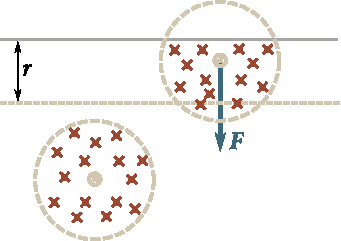
\includegraphics[scale=1.1]{figures/ch_14/fig_14_1.pdf}
		\caption[]{}
		\label{fig:14_1}
	\end{center}
	\vspace{-0.8cm}
\end{figure}

The transition of a molecule from the bulk of a liquid to its surface layer is associated with the need to do work against the forces acting in the surface layer. This work is done by the molecule at the expense of its store of kinetic energy and increases the potential energy of the molecule, just as the work done by a body flying upward against the forces of the Earth's attraction increases the potential energy of the body. When the molecule returns in to the bulk of the liquid, the potential energy which the molecule had in the surface layer transforms into the kinetic energy of the molecule.

Thus, molecules in a surface layer have an additional potential energy. The surface layer as a whole has an additional energy forming part of the internal energy of the liquid. 

Since the equilibrium position corresponds to a minimum of potential energy, a liquid left to itself will take on a shape having the minimum surface area, \ie, the shape of a sphere. What we usually observe are not liquids ``left to themselves'', but liquids subjected to the action of the Earth's gravitational forces. In this case, the liquid takes on a shape corresponding to a minimum of the total energy---that in the field of the gravitational forces and the surface energy.

When the dimensions of a body increase, its volume grows as the cube of the linear dimensions, and its surface area only as the square of these dimensions. Therefore, the energy in the gravitational field proportional to the volume of a body changes more rapidly with increasing dimensions of the body than its surface energy. In small drops of a liquid, the surface energy plays the predominate part, and as a result the drops have a shape close to a spherical one. Large drops of a liquid flatten under the action of gravitational forces notwithstanding the fact that their surface energy grows. Large bodies of a liquid take on the shape of the vessel containing them and a horizontal free surface.

The presence of surface energy causes a liquid to tend to reduce its surface area. The liquid behaves as if it were confined inside an elastic stretched out film tending to compress. It must be borne in mind that there is actually no film confining a liquid from the outside. The surface layer consists of the same molecules as the bulk of the liquid, and the interaction between the molecules in the surface layer is of the same nature as in the interior. The matter is only that the molecules in the surface layer have an additional energy in comparison with those in the bulk of the liquid.

Let us mentally separate a part of the surface of a liquid confined within a closed contour. The tendency of this portion to contract results in that it acts on the portions bordering on it with forces distributed over the entire contour (according to Newton's third law, the external portions of the surface layer act on the portion of the surface being considered with forces of the same magnitude, but opposite in direction). These forces are called forces of \textbf{surface tension}. The force of surface tension is directed along a tangent to the surface of the liquid perpendicularly to the portion of the contour it is acting upon.

Let us denote the force of surface tension per unit of length of a contour by $\sigma$. This quantity is defined as the surface tension. It is measured in newtons per metre (in the SI system) or in dynes per centimetre (in the cgs system).

\begin{figure}[t]
	\begin{center}
		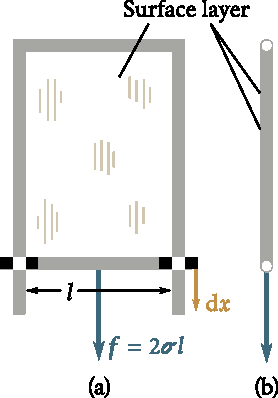
\includegraphics[scale=1.1]{figures/ch_14/fig_14_2.pdf}
		\caption[]{}
		\label{fig:14_2}
	\end{center}
	\vspace{-0.8cm}
\end{figure}

Assume that we have a rectangular frame with a movable side confining a film of a liquid (\fig{14_2}). A film is a thin flat volume of liquid confined on both sides by a surface layer (see \fig{14_2}b in which a cross section of the frame is shown). Owing to the tendency of the surface layer to contract, the film will exert a force equal to $2\sigma l$ on the movable side. For the latter to be in equilibrium, an external force $f$ must be applied to it that equals the force tensioning the film, \ie, $2\sigma l$. Let us assume that the movable side has moved very slowly in the direction of action of the force $f$ over the very small distance $\deriv{x}$. This process is attended by the liquid above the movable side doing the work $\derivp{A}=-2\sigma l\,\deriv{x}=-\sigma\,\deriv{S}$, where $\deriv{S}$ is the increment of the area of the surface layer. With such an increase of the surface, an additional number of molecules will pass from the interior of the liquid to the surface layer, losing their velocity. Therefore, if the process proceeded adiabatically, the liquid would cool slightly. We assumed, however, that the process goes on very slowly (reversibly), owing to which the temperature of the film remains constant as a result of the inflow of heat from the surroundings. Thus, the process will go on isothermally.

We established in Sec.~\ref{sec:12_6} that the work done in a reversible isothermal process equals the decrement of the free energy [see \eqn{12_56}]. We can therefore write that
\begin{equation*}
	\derivp{A} = -\sigma\,\deriv{S} = -\deriv{F}.
\end{equation*}

\noindent
The result obtained signifies that upon an isothermal increase in the area of the surface layer by $\deriv{S}$, the free energy of the liquid grows by $\deriv{F}=\sigma\,\deriv{S}$. It thus follows that the surface tension $\sigma$ is the additional free energy which a unit area of a surface layer has. Accordingly, $\sigma$ can be expressed not only in newtons per metre (or dynes per centimetre), but also in joules per square metre (or in ergs per square centimetre).

Impurities greatly affect the magnitude of the surface tension. For example, soap dissolved in water reduces its surface tension almost one-and-a-half times. When \ce{NaCl} is dissolved in water, on the contrary, the surface tension grows.

With elevation of the temperature, the difference between the densities of a liquid and its saturated vapour diminishes (see Sec.~\ref{sec:15_4}). In this connection, the surface tension also decreases. At the critical temperature (its definition is given in Sec.~\ref{sec:15_4}), $\sigma$ vanishes.

\section{Pressure under a Curved Liquid Surface}\label{sec:14_3}

Let us consider the surface of a liquid resting on a flat contour (\fig{14_3}a). If the surface of the liquid is not flat, its tendency to decrease its area leads to the appearance of a pressure apart from that exerted on a liquid with a flat surface. When the surface is convex, this additional pressure is positive (\fig{14_3}b), and when it is concave, this pressure is negative (\fig{14_3}c). In the last case, the surface layer, tending to diminish, stretches the liquid.

\begin{figure}[t]
	\begin{center}
		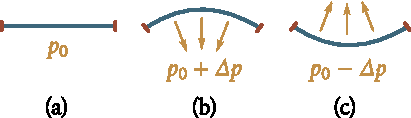
\includegraphics[scale=1.1]{figures/ch_14/fig_14_3.pdf}
		\caption[]{}
		\label{fig:14_3}
	\end{center}
	\vspace{-0.8cm}
\end{figure}

The magnitude of the additional pressure must obviously grow with an increasing surface tension $\sigma$ and surface curvature. Let us calculate the additional pressure for a spherical surface of a liquid. To do this, we shall mentally cut a spherical drop of a liquid with a diametral plane into two hemispheres (\fig{14_4}). Owing to surface tension, both hemispheres are attracted to each other with a force equal to
\begin{equation*}
	f = l\sigma = 2\pi R\sigma.
\end{equation*}

\noindent
This force presses the two hemispheres against each other over the surface $S=\pi R^2$ and, consequently, produces the additional pressure
\begin{equation}\label{eq:14_1}
	\Delta p = \frac{f}{S} = \frac{2\pi R\sigma}{\pi R^2} = \frac{2\sigma}{R}.
\end{equation}

The curvature of a spherical surface is the same everywhere and is determined by the radius of the sphere $R$. It is obvious that the smaller the radius $R$, the greater is the curvature of a spherical surface. It is customary practice to characterize the curvature of an arbitrary surface by the so-called mean curvature, which may differ for various points of a surface.

The mean curvature is determined through the curvature of normal sections. A normal section of a surface at a certain point is defined as the line of intersection of this surface with a plane passing through a normal to the surface at the point being considered. For a sphere, any normal section is a circle of radius $R$ (here $R$ is the radius of the sphere). The quantity $H=1/R$ gives the curvature of a sphere. In the general case, different normal sections passing through the same point have different curvatures. It is proved in geometry that the half-sum of the reciprocal radii of curvature
\begin{equation}\label{eq:14_2}
	H = \frac{1}{2}\parenthesis{\frac{1}{R_1} + \frac{1}{R_2}}
\end{equation}

\noindent
for any pair of mutually perpendicular normal sections has the same value. It is exactly this quantity that is the mean curvature of a surface at a given point.

The radii $R_1$ and $R_2$ in \eqn{14_2} are algebraic quantities. If the centre of curvature of a normal section is under a given surface, the relevant radius of curvature is positive; if the centre of curvature is above the surface, the radius of curvature is negative (\fig{14_5}). Thus, a curved surface can have a mean curvature equal to zero. For this purpose, the radii of curvature $R_1$ and $R_2$ must be identical in magnitude and opposite in sign.

\begin{figure}[t]
	\begin{minipage}[t]{0.5\linewidth}
		\begin{center}
			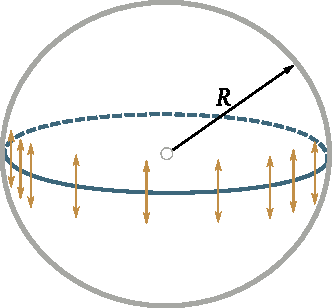
\includegraphics[scale=1]{figures/ch_14/fig_14_4.pdf}
			\caption[]{}
			\label{fig:14_4}
		\end{center}
	\end{minipage}
	\hspace{-0.05cm}
	\begin{minipage}[t]{0.5\linewidth}
		\begin{center}
			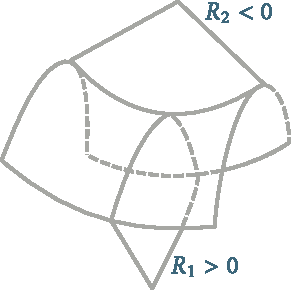
\includegraphics[scale=1]{figures/ch_14/fig_14_5.pdf}
			\caption[]{}
			\label{fig:14_5}
		\end{center}
	\end{minipage}
	\vspace{-0.4cm}
\end{figure}

For a sphere, we have $R_1=R_2=R$, so that by \eqn{14_2}, $H=1/R$. Substituting $H$ for $1/R$ in \eqn{14_1}, we get
\begin{equation}\label{eq:14_3}
	\Delta p = 2H\sigma.
\end{equation}

The French scientist Pierre Laplace (1749-1827) proved that \eqn{14_3} holds for a surface of any shape if by $H$ we understand the mean curvature of a surface at the point under which the additional pressure is being determined. Introducing the expression~\eqref{eq:14_2} for the mean curvature into \eqn{14_3}, we get a formula for the additional pressure under an arbitrary surface:
\begin{equation}\label{eq:14_4}
	\Delta p = \sigma\parenthesis{\frac{1}{R_1} + \frac{1}{R_2}}.
\end{equation}

\noindent
It is called the \textbf{Laplace formula}.

The additional pressure given by \eqn{14_4} causes the level of a liquid in a narrow tube (capillary) to change. This is why it is sometimes called the \textbf{capillary pressure}.

\section{Phenomena on Liquid-Solid Interface}\label{sec:14_4}

Everything said in Sec.~\ref{sec:14_2} about the special conditions in which the molecules of a surface layer are also relates completely to solids. Hence, solids, like liquids, have a surface tension.

When considering phenomena on the interface between various media, we must not forget that the surface energy of a liquid or solid depends not only on the properties of the given liquid or solid, but also on the properties of the substance with which they have a common boundary. Strictly speaking, we must consider the total surface energy $\sigma_{12}$ of both substances in contact with each other (\fig{14_6}). Only if one of the substances is gaseous, does not react chemically with the other substance, and has a poor solubility in it, can we simply speak of the surface energy (or the surface tension) of the second liquid or solid.

\begin{figure}[t]
	\begin{minipage}[t]{0.5\linewidth}
		\begin{center}
			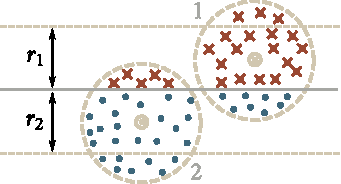
\includegraphics[scale=1]{figures/ch_14/fig_14_6.pdf}
			\caption[]{}
			\label{fig:14_6}
		\end{center}
	\end{minipage}
	\hspace{-0.05cm}
	\begin{minipage}[t]{0.5\linewidth}
		\begin{center}
			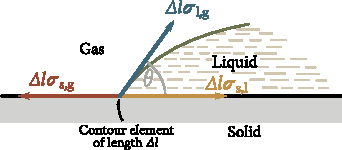
\includegraphics[scale=1]{figures/ch_14/fig_14_7.pdf}
			\caption[]{}
			\label{fig:14_7}
		\end{center}
	\end{minipage}
	\vspace{-0.4cm}
\end{figure}

If three substances, namely, a solid, a liquid, and a gas, are in direct contact with one another (\fig{14_7}), then the entire system takes on a configuration corresponding to the minimum of the total energy (surface, in the field of forces of gravity, etc.) In particular, the contour along which the three substances are in contact is arranged on the surface of the solid so that the sum of the projections of all the surface tension forces applied to each contour element onto the direction in which the contour element can move (\ie, onto a direction tangent to the surface of the solid) equals zero. It can be seen from \fig{14_7} that the condition of equilibrium of a contour element of length $\Delta l$ is
\begin{equation}\label{eq:14_5}
	\Delta l \ab{\sigma}{s,g} = \Delta l \ab{\sigma}{s,l} + \Delta l \ab{\sigma}{l,g}\cos\theta
\end{equation}

\noindent
where $\ab{\sigma}{s,g}, \ab{\sigma}{s,l}$ and $\ab{\sigma}{l,g}$ are the surface tensions at the solid-gas, solid-liquid, and liquid-gas interfaces.

The angle $\theta$ measured inside the liquid between tangents to the surface of the solid and the surface of the liquid is called the \textbf{contact angle}. In accordance with \eqn{14_5}, we have
\begin{equation}\label{eq:14_6}
	\cos\theta = \frac{\ab{\sigma}{s,g} - \ab{\sigma}{s,l}}{\ab{\sigma}{l,g}}.
\end{equation}

\noindent
The contact angle is determined by \eqn{14_6} only provided that
\begin{equation}\label{eq:14_7}
	\frac{|\ab{\sigma}{s,g} - \ab{\sigma}{s,l}|}{\ab{\sigma}{l,g}} \leqslant 1.
\end{equation}

\noindent
If this condition is not observed, \ie, $|\ab{\sigma}{s,g} - \ab{\sigma}{s,l}|>\ab{\sigma}{l,g}$, then equilibrium cannot set in at any value of $\theta$. This occurs in two cases.
\begin{enumerate}[1.]
	\item $\ab{\sigma}{s,g}>\ab{\sigma}{s,l}+\ab{\sigma}{l,g}$. No matter how small the angle $\theta$ is, the	force $\ab{\sigma}{s,g}$ overbalances the other two (\fig{14_8}a). In this case, the liquid flows unlimitedly over the surface of the solid---\textbf{complete wetting} takes place. The replacement of a solid-gas interface with two interfaces-solid-liquid and liquid-gas ones---is advantageous from the energy viewpoint. The contact angle is zero in complete wetting.
	
	\item $\ab{\sigma}{s,l}>\ab{\sigma}{s,g}+\ab{\sigma}{l,g}$. No matter how close to $\pi$ the angle $\theta$ is, the force $\ab{\sigma}{s,l}$ overbalances the other two (\fig{14_8}b). In this case, the liquid-solid interface contracts into a point, and the liquid separates from the surface of the solid---\textbf{complete non-wetting} takes place. The replacement of a solid-liquid interface with two interfaces---solid-gas and liquid-gas ones---is advantageous from the energy viewpoint. In complete non-wetting, the contact angle is $\pi$.
\end{enumerate}

\begin{figure}[t]
	\begin{center}
		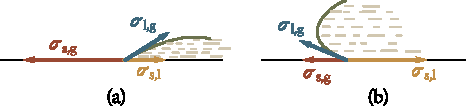
\includegraphics[scale=1.1]{figures/ch_14/fig_14_8.pdf}
		\caption[]{}
		\label{fig:14_8}
	\end{center}
	\vspace{-0.75cm}
\end{figure}

When condition~\eqref{eq:14_7} is observed, the contact angle may be acute or obtuse depending on the relation between $\ab{\sigma}{s,g}$ and $\ab{\sigma}{s,l}$. If $\ab{\sigma}{s,g}$ is greater than $\ab{\sigma}{s,l}$ then $\cos\theta>0$ and the angle $\theta$ is acute (\fig{14_9}a). In this case, partial wetting occurs. If $\ab{\sigma}{s,g}$ is smaller than $\ab{\sigma}{s,l}$ then $\cos\theta<0$ and the angle $\theta$ is obtuse (\fig{14_9}b). In this case, partial non-wetting occurs.

Non-wetting may result in interesting phenomena. It is general knowledge that a needle or safety razor blade coated with grease can float on the surface of water. It is very simple to explain this, at first sight, curious phenomenon on the basis of energy considerations. The greased surface of steel is not wetted by water; the steel-water interface has a much greater energy than the steel-air or air-water ones. The complete submersion of a needle into water is attended by an increase in the surface energy from $S\ab{\sigma}{s,g}$ (steel-air) to the value $S\ab{\sigma}{s,l}$ (steel-water), where $S$ is the surface area of the needle. The change in the surface energy upon submersion is described by the curve $\ab{E}{sur}$ shown in \fig{14_10}. The symbol $h$ stands for the height of the needle above the bottom of the vessel, $h_0$ is the height of the surface of the liquid above the bottom of the vessel. The dependence of the potential energy of the needle in the field of the Earth's gravitation $\ab{E}{gr}$ on $h$ has the form of a straight line passing through the origin of coordinates. The total energy $\ab{E}{tot}=\ab{E}{sur}+\ab{E}{gr}$ has a minimum when $h=h_0$. This is exactly what permits the needle to float on the surface of the water. If we press on the needle and submerge it to a depth such that the total energy passes through its maximum and begins to decrease, then the needle will submerge further by itself and sink.

\begin{figure}[t]
	\begin{minipage}[t]{0.5\linewidth}
		\begin{center}
			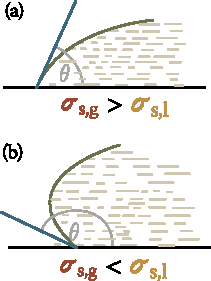
\includegraphics[scale=0.95]{figures/ch_14/fig_14_9.pdf}
			\caption[]{}
			\label{fig:14_9}
		\end{center}
	\end{minipage}
	\hspace{-0.05cm}
	\begin{minipage}[t]{0.5\linewidth}
		\begin{center}
			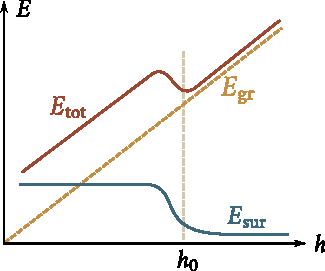
\includegraphics[scale=0.95]{figures/ch_14/fig_14_10.pdf}
			\caption[]{}
			\label{fig:14_10}
		\end{center}
	\end{minipage}
	\vspace{-0.3cm}
\end{figure}

\begin{figure}[t]
	\begin{center}
		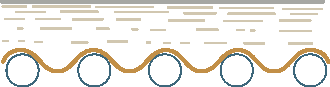
\includegraphics[scale=0.95]{figures/ch_14/fig_14_11.pdf}
		\caption[]{}
		\label{fig:14_11}
	\end{center}
	\vspace{-0.9cm}
\end{figure}

The possibility of ``carrying water in a sieve'' is explained in a similar way. If water does not wet a sieve (this can be achieved by coating the wires forming the sieve with paraffin) and the layer of water is not very thick, then a slight displacement of the water level downward (\fig{14_11}) will be attended by an increase in the surface energy exceeding in magnitude the decrease in the energy in the field of gravitational forces. Hence, the water will be retained in the sieve and will not spill out.

\section{Capillary Phenomena}\label{sec:14_5}

The existence of the contact angle leads to curvature of the surface of a liquid near the walls of the vessel containing it. In a narrow tube (capillary\footnote{The Latin \textit{capillus} means hair. A capillary is a ``tube as thin as a hair''.}) or in a narrow gap between two walls, the entire surface is curved. If the liquid wets the walls, the surface is concave, and if it does not wet them, the surface is convex (\fig{14_12}). Such curved surfaces of a liquid are called meniscuses.

If one end of a capillary is immersed in a liquid poured into a broad vessel, then the pressure under the curved surface in the capillary will differ from that under the flat surface in the broad vessel by the amount $\Delta p$ determined by \eqn{14_4}. As a result, the level of the liquid in the capillary will be higher than in the vessel if the liquid wets it, and lower if the liquid does not wet it.

The change in the height of the liquid level in narrow tubes or gaps has been named \textbf{capillarity}. In the broad meaning of the term, capillary phenomena are understood to include all the phenomena due to the existence of surface tension. In particular, the pressure expressed by \eqn{14_4} and due to surface tension is called, as we have already indicated, capillary pressure. 

A difference $h$ sets in between the level of a liquid in a capillary and in a broad vessel such that the hydrostatic pressure $\rho gh$ is balanced by the capillary pressure $\Delta p$:
\begin{equation}\label{eq:14_8}
	\rho gh = \frac{2\sigma}{R}.
\end{equation}

\noindent
In this equation, $\sigma$ is the surface tension on the liquid-gas interface, and $R$ is the radius of curvature of the meniscus. The latter can be expressed through the contact angle $\theta$ and the radius of the capillary $r$. Indeed, examination of \fig{14_12} shows that $R=r/\cos\theta$. Using this value in \eqn{14_8} and solving the equation obtained relative to $h$, we arrive at the equation
\begin{equation}\label{eq:14_9}
	h = \frac{2\sigma\cos\theta}{\rho gr}.
\end{equation}

In accordance with the fact that a wetting liquid rises in a capillary, while a non-wetting liquid lowers in it, \eqn{14_9} gives a positive $h$ for $\theta<\pi/2$ (because $\cos\theta>0$), and a negative $h$ for $\theta>\pi/2$ (because $\cos\theta<0$).

In deriving \eqn{14_9}, we assumed that the meniscus has a spherical shape. The equation for $h$ can also be obtained on the basis of energy considerations, and there is no need to make a special assumption on the shape of the meniscus. The equilibrium position of the meniscus will correspond to a minimum energy $E$ of the liquid-capillary system. This energy consists of the surface energy on the liquid wall, liquid-gas, and wall-gas interfaces, and also of the potential energy of the liquid in the field of the Earth's gravitation.

\begin{figure}[t]
	\begin{minipage}[t]{0.5\linewidth}
		\begin{center}
			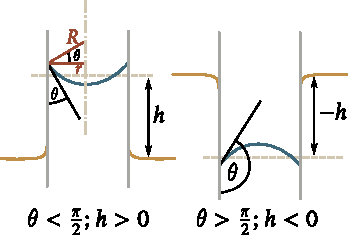
\includegraphics[scale=0.95]{figures/ch_14/fig_14_12.pdf}
			\caption[]{}
			\label{fig:14_12}
		\end{center}
	\end{minipage}
	\hspace{-0.05cm}
	\begin{minipage}[t]{0.5\linewidth}
		\begin{center}
			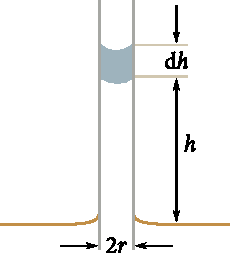
\includegraphics[scale=0.95]{figures/ch_14/fig_14_13.pdf}
			\caption[]{}
			\label{fig:14_13}
		\end{center}
	\end{minipage}
	\vspace{-0.4cm}
\end{figure}

Let us find the increment of the energy dE corresponding to an increment of the height $\deriv{h}$ to which a liquid rises in a capillary. When the height grows to $\deriv{h}$, the surface area of contact of the liquid with the wall of the capillary increases by $2\pi r\,\deriv{h}$, owing to which the energy receives an increment of $2\pi r\ab{\sigma}{s,l}\,\deriv{h}$. Simultaneously, the surface area of contact between the wall and the gas diminishes, which is attended by an increment of the energy of $-2\pi r\ab{\sigma}{s,g}\,\deriv{h}$. The potential energy in the field of the Earth's gravitation acquires an increment equal to the force of gravity acting on the shaded volume of the liquid (\fig{14_13}) multiplied by $h$, \ie, equal to $g\rho\pi r^2h\,\deriv{h}$. We may disregard the change in the level of the liquid in the broad vessel. Thus,
\begin{equation*}
	\deriv{E} = 2\pi r\parenthesis{\ab{\sigma}{s,l} - \ab{\sigma}{s,g}}\,\deriv{h} + g\rho\pi r^2h\,\deriv{h}.
\end{equation*}

\noindent
Hence,
\begin{equation*}
	\diff{E}{h} = 2\pi r\parenthesis{\ab{\sigma}{s,l} - \ab{\sigma}{s,g}} + g\rho\pi r^2h.
\end{equation*}

\noindent
Equating this derivative to zero, we obtain the condition of equilibrium, from which it follows that
\begin{equation}\label{eq:14_10}
	h = \frac{2\parenthesis{\ab{\sigma}{s,l} - \ab{\sigma}{s,g}}}{g\rho r}.
\end{equation}

\noindent
According to \eqn{14_6}, $\ab{\sigma}{s,l} - \ab{\sigma}{s,g} = \ab{\sigma}{l,g}\cos\theta$. Making this substitution in \eqn{14_10} and using simply $\sigma$ instead of $\ab{\sigma}{l,g}$ we get \eqn{14_9}.

